\section{Durchführung}
\label{sec:Durchführung}

\subsection{Versuchsaufbau}

In \autoref{fig:aufbau} findet sich eine beschriftete Version des verwendeten Aufbaus.

\begin{figure}{H}
    \centering
    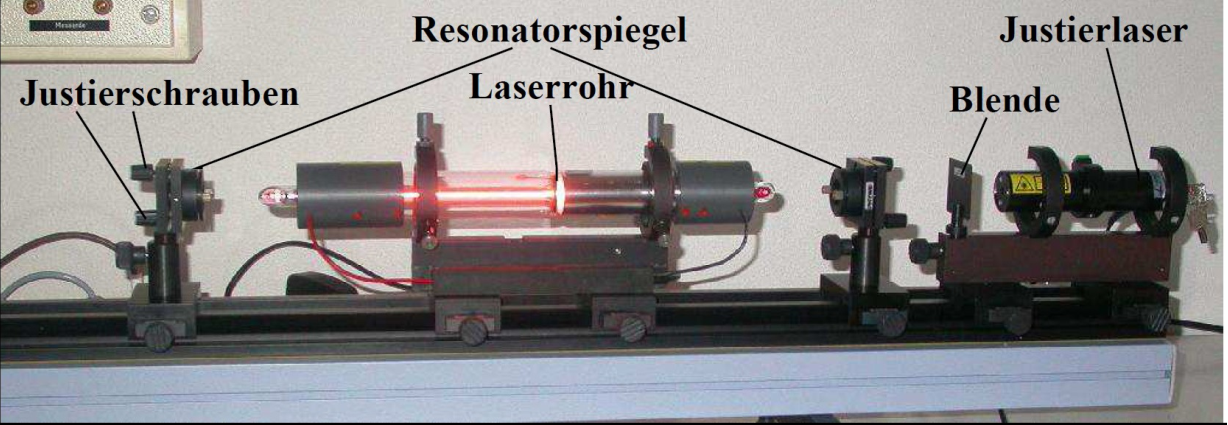
\includegraphics[width=\textwidth]{figures/Aufbau.pdf}
    \caption{Beschrifteter Aufbau des Versuches \cite{v61}.}
    \label{fig:aufbau}
\end{figure}

Zusätzlich zu den in \autoref{fig:aufbau} beschriebenen Komponenten stehen eine Photodiode, ein Draht, ein Polarisator, einige Gitter sowie die in \autoref{fig:spiegel} aufgeführten Spiegel zur Resonatorkonfiguration
zur Verfügung.

\begin{figure}[H]
    \centering
    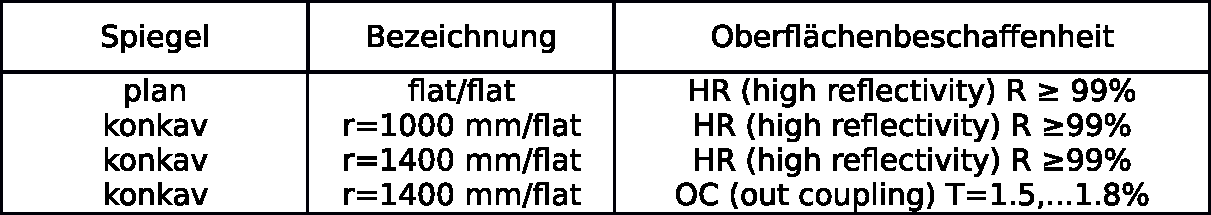
\includegraphics[width=\textwidth]{figures/Spiegel.pdf}
    \caption{Aufführung der zum Aufbau des Resonators zur Verfügung stehenden Spiegel \cite{v61}.}
    \label{fig:spiegel}
\end{figure}

\subsection{Messprogramm}

Im Folgenden wird näher auf die einzelnen Schritte des Messprozesses eingegangen.

\subsubsection{Justage des Lasers}

Die Justage des Lasers ist bereits vor Beginn des Versuches durchgeführt worden.
Da in den folgenden Messschritten der Laserstrahl jedoch einige Male neu justiert werden muss, soll hier dennoch darauf eingegangen werden. \\

Die Hochspannung wird auf $6,5 \,\unit{\ampere}$ gestellt, bevor begonnen wird. \\
Zur Hilfe steht ein bereits vorjustierter grüner Laser und einige Targets bereit.
Um den HeNe-Laser zu justieren, wird der grüne Laser angeschaltet und die Resonatorspiegel so justiert, dass der grüne Strahl genau durch die Targets zurück auf den grünen Laser fällt.
Werden dann die Targets aus dem Strahl entfernt, sollte der HeNe-Laser justiert sein.

\subsubsection{Überprüfen der Stabilitätsbedingung}

Zur Überprüfung der Stabilitätsbedingung wird die Resonatorlänge variiert und mithilfe einer Photodiode der Photostrom gemessen. Es handelt sich um eine rein qualitative Messreihe, bei der überprüft wird,
bis zu welcher Resonatorlänge der Strahl stabil bleibt. 
Diese Messreihe wird einmal mit einem plan-konkaven und einmal mit einem konkav-konkav Resonator durchgeführt. \\

Um Zeit zu sparen wird diese Messung mit der Messung des Frequenzspektrums kombiniert.


\subsubsection{Beobachten der $TEM$-Moden}

Zur Messung der $TEM_{00}$-Mode wird zunächst eine Streulinse in den Strahl eingeführt, die das Muster auf dem optischen Schirm deutlicher macht.
Zur Vermessung wird eine Photodiode zwischen Laser und optischen Schirm gestellt und auf der Horizontalen verschoben.
Dann wird zwischen Laserrohr und Resonatorspiegel ein dünner Draht gebracht und der Prozess wiederholt.


\subsubsection{Bestimmung der Polarisation}

Um die Polarisation des Lasers zu bestimmen, wird zwischen Schirm und Laser ein Polarisator positioniert.
Dann wird in Abständen von $5 \, °$ der Winkel justiert und der gemessene Photostrom notiert.


\subsubsection{Multimodenbetrieb und Frequenzspektrum}

Für unterschiedliche Resonatorlängen wird die Schwebung des Multimodenspektrums des Lasers mithilfe eines Frequenzanalysators gemessen. 
Dazu wird eine schnelle Photodiode verwendet.


\subsubsection{Bestimmung der Wellenlänge}

Schließlich wird noch die Wellenlänge des Lasers bestimmt.
Dazu werden Gitter unterschiedlicher Gitterkonstanten zwischen den Schirm und Laser gestellt.
Mithilfe eines Maßbandes werden dann die Abstände der Maxima des entstehenden Interferenzmusters vermessen.